%====================================================================================================
% ?????
%====================================================================================================
% TCC
%----------------------------------------------------------------------------------------------------
% Autor				: Jasane Schio
% Orientador		: Gedson Faria
% Co-Orientador		: Angelo Darcy
% Instituição 		: UFMS - Universidade Federal do Mato Grosso do Sul
% Departamento		: CPCX - Sistema de Informação
%----------------------------------------------------------------------------------------------------
% Data de criação	: 01 de Outubro de 2015
%====================================================================================================
% Define o caminho das figuras
\graphicspath{{figuras/}}
\chapter{Fundamentação Teórica} \label{Cap:Fundamentacao}

%\section{Estado da Arte} \label{Sec:EstadoDaArte}
%Como estado da arte foram relacionados os métodos de detecção de objetos em imagens em tempo real e estáticas.

\section{Processamento de Imagens}
\subsection{Detecção de Objetos}
\label{Sec:TiposDeDeteccaoDeObjetos}
Antes de descrever os métodos de classificação devemos fazer algumas definições:
\begin{itemize}
	\item	Em cada detecção de objetos são obtidas as informações sobre a imagem, essas são de acordo com o tipo de detecção desejada. Os dados podem conter informações como posição, tamanho, borda, transformação linear, rotação entre outros. Cada detecção em uma imagem é chamada de pose.
	
	\item	Métodos de detecção de objeto baseado em classes constroem a classe do objeto baseada em um conjunto de treino. O conjunto de treino é composto por múltiplas imagens exemplo do objeto para que seja assim capturado os aspectos do objeto.
\end{itemize}

A detecção de objetos pode ser considerada uma técnica herdada do reconhecimento de padrões da área de aprendizado de máquina, esta consiste em separar objetos por categorias de acordo com uma ou mais características especificas. Quando essa técnica se junta ao processamento de imagens, onde são acentuadas as características especificas do objeto dentro da imagem para assim este se destacar, tornou-se possível a detecção de objetos em imagens que dentro do campo de visão computacional é uma das áreas que mais obtêm a atenção de pesquisadores. O primeiro Framework de métodos que usam base de dados categorizando uma ou mais características de um objetos para fazer o reconhecimento através de aprendizado foi apresentado em 2001 por Viola e Jones\cite{Viola:2001}. Desde o framework de Viola e Jones até os dias atuais muitos métodos e teorias para detecção já foram propostos e implementados como detecção de faces utilizando um classificador de redes neurais na intensidade de padrões de uma imagem, support vector machine para localizar rostos humanos e carros\cite{Nascimento:2007}, análise de componentes principais, análise independente de componentes, fatoração de matriz não-negativa, análise discriminativa linear, boosting\cite{Roth:2008}, além da classificação binaria, onde se considera a detecção do objeto em tamanho fixo apenas variando na posição na imagem\cite{AmitFelzenszwalb:2014}. 

Em 2005 Ulusoy e Bishop\cite{Ulusoy:2005} mostraram o quão útil seria categorizar os métodos de detecção de imagens, e os dividiram em duas principais categorias: generativa e discriminativa. Categorias que foram aceitas e utilizadas como mostram Amit e Falzenszwalb\cite{AmitFelzenszwalb:2014} e Roth e Winter\cite{Roth:2008}.

O método generativo pode ser descrito como um modelo probabilístico para a variância da pose de um objeto juntando com o modelo de aparência, ou seja, um modelo de probabilidade para a aparência da imagem condicional em uma determinada pose, juntamento com um modelo de fundo. Os parâmetros do modelo são estimados a partir de dados retirados de treinamento e as decisões são baseadas nas probabilidades anteriores\cite{AmitFelzenszwalb:2014}. Em resumo o método generativo tenta encontrar uma representação adequada dos dados originais através da aproximação dos dados originais, mas mantendo o máximo de informação possível\cite{Roth:2008}.

Já o modelo discriminativo tipicamente constrói um classificador que pode discriminar entre imagens (ou sub-imagens) contendo o objeto e as que não contém o objeto. Os parâmetros do classificador são selecionados para minimizar os erros nos dados de treino\cite{AmitFelzenszwalb:2014}.


%	Ulusoy\cite{Ulusoy:2005} apontou as principais vantagens dos dois metodos. 
Segundo Ulusoy e Bishop\cite{Ulusoy:2005} o método generativo se destaca por tratar perda de dados ou dados parcialmente rotulados, pela facilidade em que uma nova classe pode ser incrementada na classificação condicional de densidade, independentemente das classes anteriores, e por conseguir facilmente lidar com composição de objetos (ex: óculos, chapéus...), considerando que os modelos discriminativos precisar analisar todas as combinações durante o treinamento. Amit e Felzenszwalb\cite{AmitFelzenszwalb:2014} ainda aponta que as vantagens descritas sobre o método discriminativo são ditas como a flexibilidade do modelo  que pode ser utilizado em regiões do espaço de entrada onde as probabilidades posteriores diferem significativamente de 0 ou 1, ao passo que as abordagens detalhes generativas modelo de distribuição de X, que podem ser irrelevantes para determinar as probabilidades posteriores, além de ser tipicamente muito rápido em fazer previsões para os novos pontos (teste) de dados, enquanto os modelos generativos muitas vezes exigem solução iterativa, e pela igualdade de circunstâncias, seria de esperar que os métodos discriminativos tenham melhor desempenho preditivo, uma vez que são treinados para prever o rótulo de classe em vez de a distribuição conjunta de vetores e alvos de entrada.

\subsection{Detecção de Bordas}
Para um objeto poder ser detectado por algum método de detecção de objetos a imagem passa por um processo de segmentação. A segmentação pode ser dita como o processo de divisão da imagem em objetos\cite{Gonzalez:2008}. De acordo com Wangenheim\cite{Wangenheim:2014} o processo de segmentação se baseia em dois conceitos: similaridade e descontinuidade. A descontinuidade é o processo onde se separa o fundo das partículas e estas umas das outras, através de linhas, bordas ou pontos. Já a similaridade é o processo onde os pixeis provenientes da descontinuidade são agrupados de acordo com a proximidade um dos outros para formar os objetos de interesse. De acordo com Canny\cite{Canny:1986} o processo de detecção de bordas é um processo simplificado que serve para diminuir drasticamente o total de dados a serem processados e ao mesmo que o mesmo preserva informações valiosas sobre os objetos. É muito comum a ocorrência de ruídos quando se trata da detecção de bordas, e por sua vez para evitar esses ruídos é necessário a suavização da imagem antes de fazer a detecção. Vale\cite{Vale:2002} lembra que a suavização possui pontos negativos como perda de informação e deslocamento de estruturas de feições proeminentes no plano da imagem. Além disso, existem diferenças entre as propriedades dos operadores diferenciais comumente utilizados, o que ocasiona  bordas diferentes.Assim, como dito por Ziou e Tabbone citados por Vale\cite{Vale:2002}, se torna difícil encontrar um algoritmo que tenha bom desempenho em diferenciados contextos e capture os requisitos necessários aos estágios subsequentes do processamento. 
Quando se trata de detecção de bordas existem dois critérios\cite{Canny:1986} para essa detecção que devem ser levados em consideração, Taxa de Erro e Localização\cite{Vale:2002}. 
\begin{description}
	\item[Taxa de Erro] É importante que as bordam contidas na imagem não sejam confundidas ou perdidas e ainda que não sejam detectadas bordas falsas. É necessário que o algoritmo de detecção de borda tenha uma baixa taxa de erro para que seja eficiente.\cite{Wangenheim:2014, Canny:1986, Vale:2002}
	\item[Localização] A distância entre os pixels de borda encontradas pelo algoritmo e a borda atual deveriam ser o menor possível.\cite{Wangenheim:2014}
\end{description}
Ao tentar aplicas esses dois critérios para desenvolver um modelo matemático para detecção de bordas sem a necessidade de base em regras preestabelecidas em seu artigo
\textit{ A Computational Approach to Edge Detection} Canny percebeu que somente esses dois critérios não eram o suficiente para obter uma boa precisão da detecção de bordas. E então propôs um terceiro critério: Resposta.
\begin{description}
	\item[Resposta] Para contornar a possibilidade de mais de uma resposta para a mesma borda, ou seja o detector de bordas não deveria identificar múltiplos pixels de borda onde somente exista um único pixel. \cite{Wangenheim:2014, Canny:1986, Vale:2002}
\end{description}

Com o acréscimo do terceiro critério então nota-se que o processo de detecção de bordas de Canny
mostrou-se bastante flexível, independente da origem da imagem utilizada\cite{Vale:2002}.









\section{Espaço e Modelo de Cores} \label{Sec:Cores}


O olho humano é capaz de identificar cores mesmo com as mais diferentes interferências, luminosidade, tonalidade, intensidade, entre outras ações de agentes externos, pois nosso cérebro assimila a cor a sua aparência, já para uma máquina cores são números, códigos, cada cor contém um código especifico e cada uma de suas variâncias e alterações também. Para o nosso cérebro é muito fácil entender, exemplo, que o verde, verde lima, verde escuro são a mesma cor, apenas com tonalidades diferentes, já para o computador estas são: (0,255,0),(50,205,50),(0,128,0), no padrão de cor RGB que considera uma luz visível. Mas se for aplicado luminosidade nessas cores, por exemplo, elas ainda se tornam outras diferentes cores, um código diferente para cada luminosidade possível. Para conseguir cobrir todas essas alterações nas cores foram definidos em 1921 começaram então pela Comissão Internacional de Iluminação (CEI) a serem definidos espaços e modelos de cores\cite{Souto:2003}.

\subsection{Espaços de Cores}
Segundo Foley et. al citado por Souto\cite{Souto:2003} espaço de cores é um sistema tridimensional de
coordenadas, onde cada eixo refere-se a uma cor primária. A quantidade de cor primária
necessária para reproduzir uma determinada cor, é atribuída a um valor sobre o eixo
correspondente. O espaço de cores pode ser entendido como a quantidade de detalhamento, tonalidades de uma cor, dentro do espectro de cores de um determinado modelo de cor. 
Quando fez sua primeira experiência com a decomposição da luz em um prisma para obter cores Newton percebeu que não havia a cor branca. Ele tentou então misturar as sete cores que obteve para gerar a branca, sem sucesso. Parar gerar a cor branca é necessário a soma das três cores primarias azul, verde e vermelho. Apos anos de estudo entendeu-se que existe duas formas de se obter cores: através da emissão ou reflexão de luz, espaços RGB e CMY respectivamente, \figurename{ 2.2}. 

\subsubsection{RGB}
O espaço de cores que emitem luz é conhecido como RGB que é baseado na teoria das cores primarias vermelho, verde e azul, em inglês Red, Green, Blue, para simular a tricromática visão humana, onde toda cor é composta pela soma das três cores.
\subsubsection{CMY}
O espaço de cores que refletem luz é conhecido como CMY que são as cores ciano, magenta e amarelo, em inglês Cyan, Magenta e Yellow. Neste espaço a cor é obtida pela subtração das cores. Existe uma variação ao CMY chamada de CMYK onde é acrescentada a cor preta e foi criado 	como uma opção mais barata, pois não necessita de pigmentos puros\cite{Rocha:2010}.
\newline
\begin{figure}[!h]
	\centering
	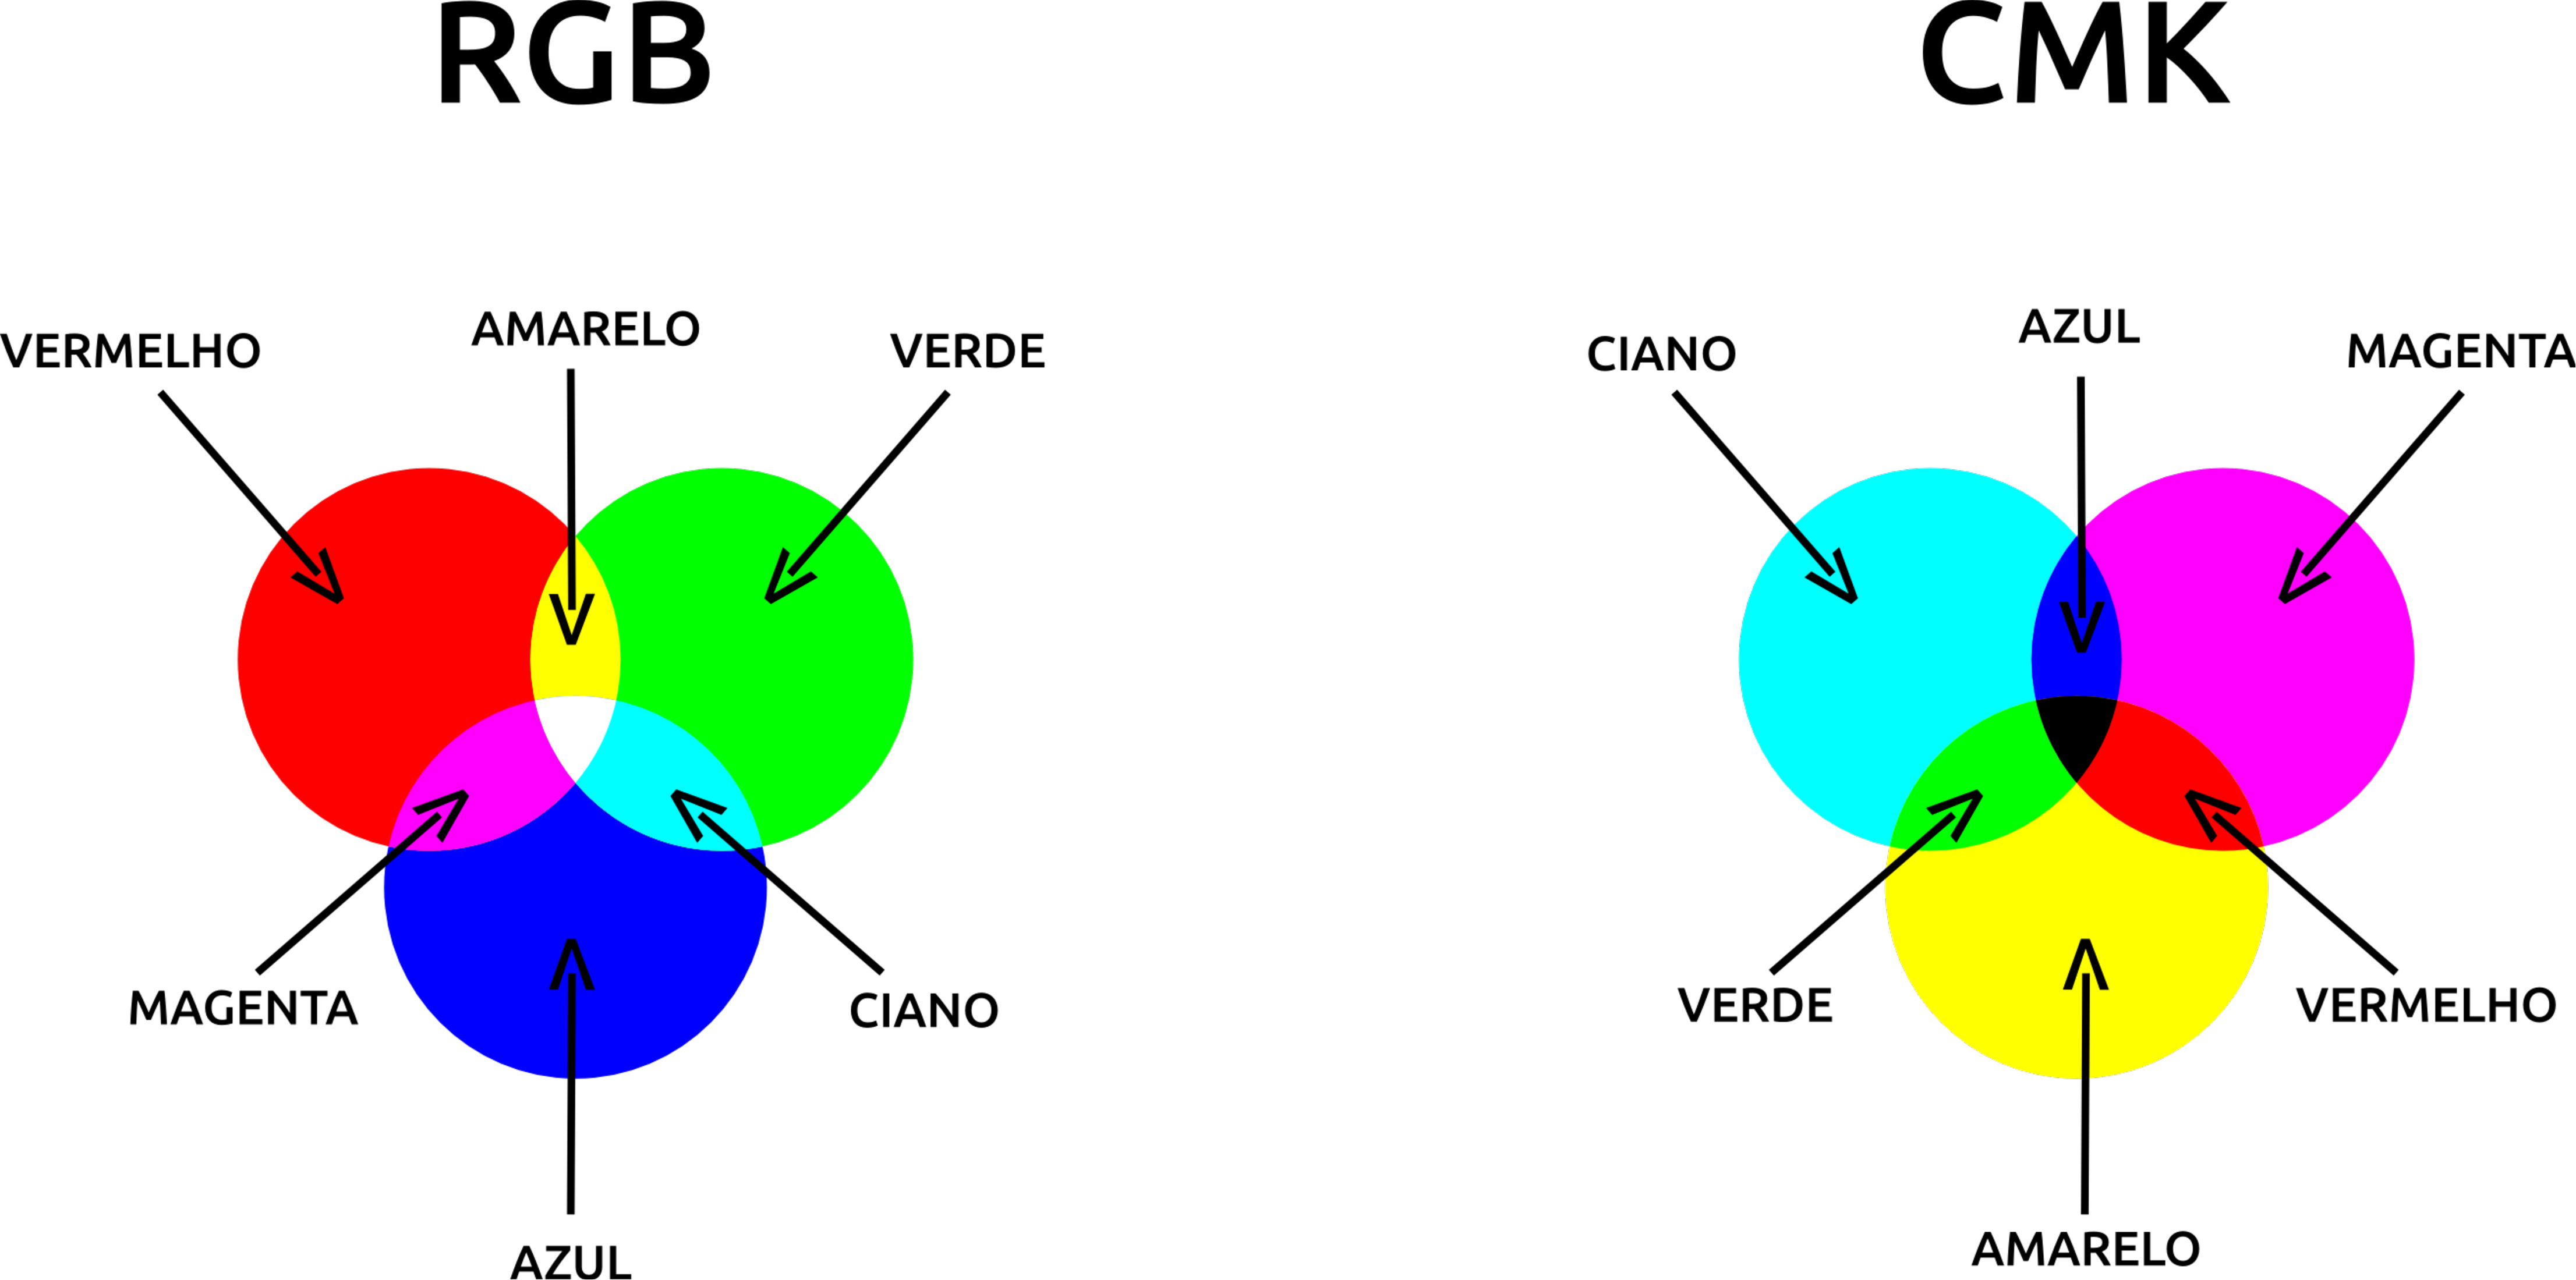
\includegraphics[width=0.8\textwidth]{espacos.pdf}
	\caption{Exemplo dos espaços de cores RGB E CMY.}
	\label{Espaco de Cores}
\end{figure}
\subsection{Modelo de Cores}
Modelo de cores são modelos matemáticos utilizados para classificação das cores de acordo com sua tonalidade, saturação, luminosidade ou crominância na tentativa de conseguir cobrir o maior número de cores possíveis e assim simulando a visão. A representação da cor é definida por um único ponto em um modelo tridimensional. 
\subsubsection{RGB}
O modelo de cores RGB pode ser considerado mais básico dos modelos de cores. Seu nome possui a mesma definição do espaço de cores RGB. Ele não utiliza de nenhum atributo como luminosidade ou tonalidade, por exemplo, para a definição da cor apenas a adição das cores primarias, azul, verde e vermelho. É este também o padrão mais usado e conhecido. Os valores de R,G e B variam de 0 à 255.
\begin{figure}[!h]
	\centering
	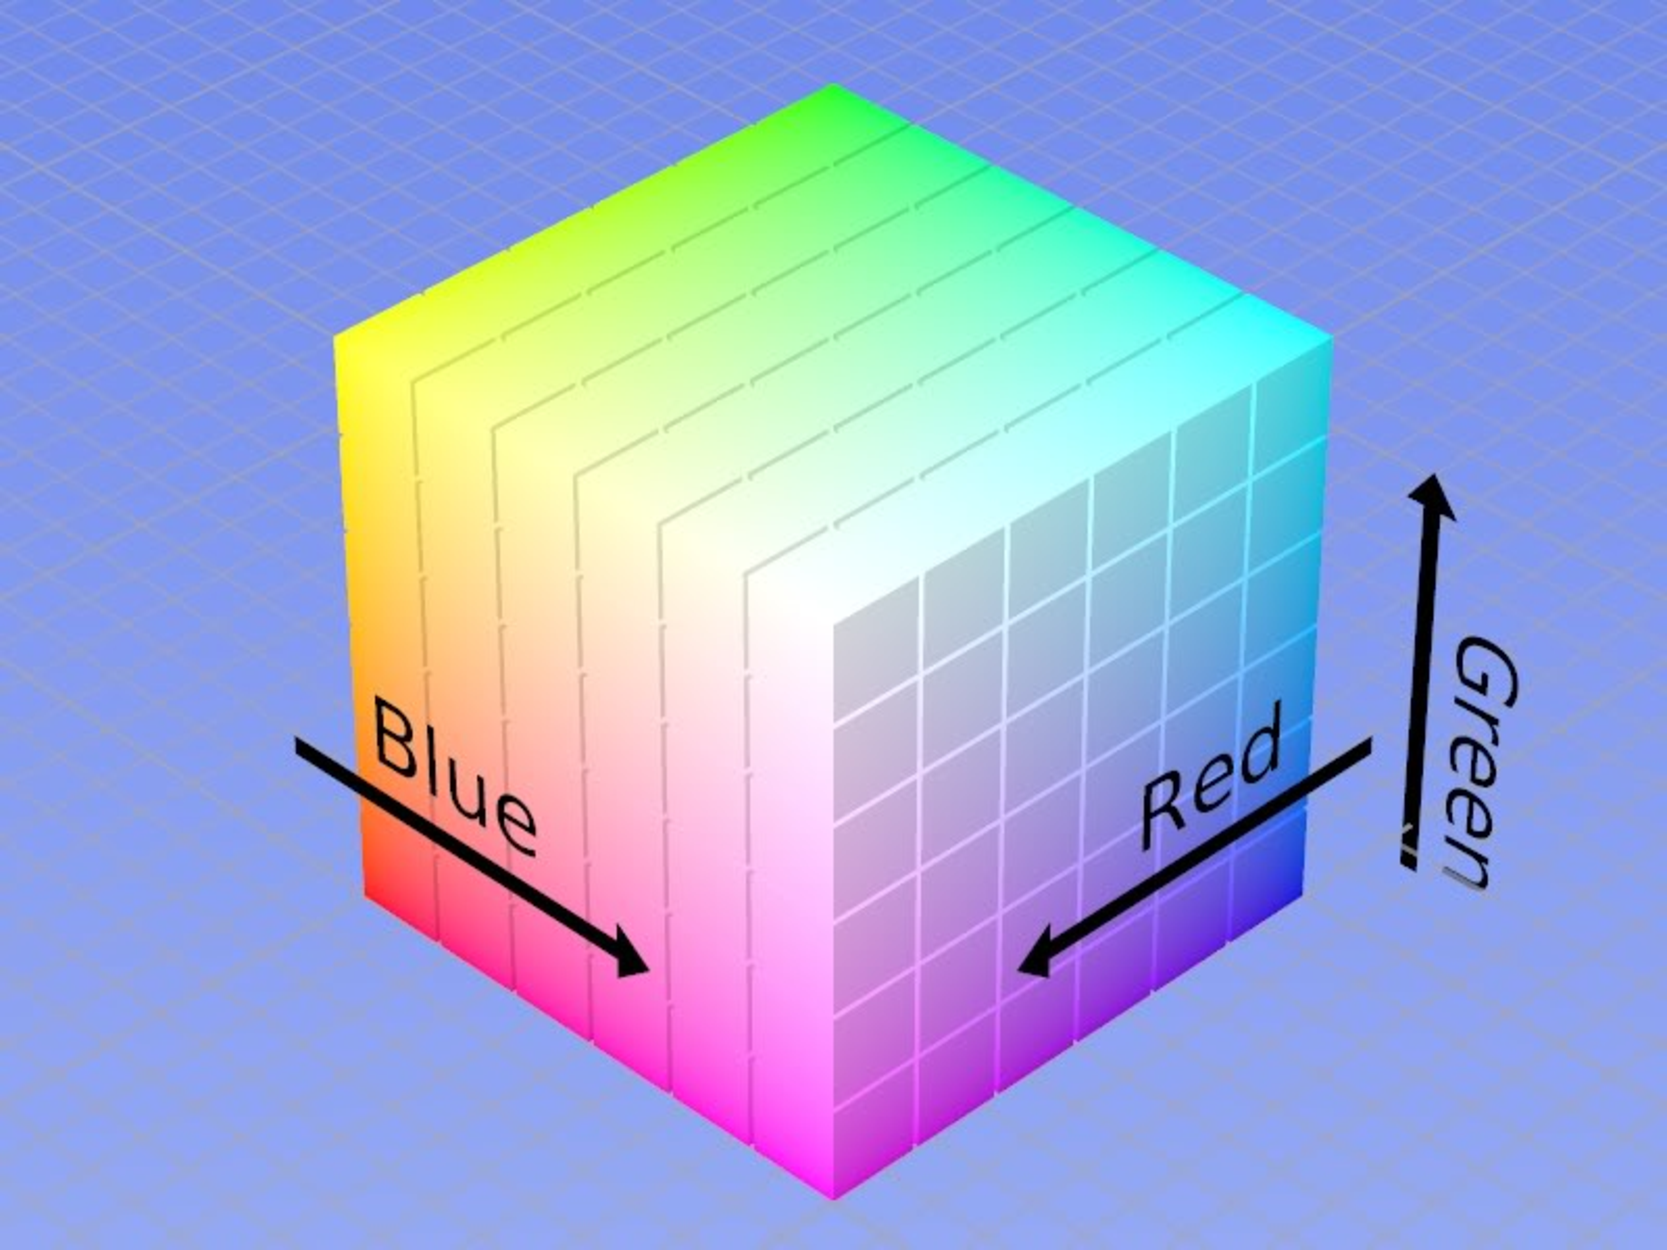
\includegraphics[width=0.5\textwidth]{rgb.pdf}
	
	\caption{Exemplo do Modelo de Cor RGB.	 Horvath\cite{ImagensHSLHSVRGB}  }
	\label{ModeloRGB}
\end{figure}
\subsubsection{HSL, HSB/HSV}
Os modelo de cores tem função definir as cores nos programas gráficos de computadores de forma que combine com a 
percepção das cores pelo sistema visual humano e utiliza três eixos similares para definirem a cor\cite{Leao:2005}.
O modelo HSL define tonalidade (hue) que é a cor em si, variando de 0 a 360º, saturação (saturnation) que define o grau de pureza da cor, obtido pela mistura da tonalidade com a cor cinza,variando de 0 a 1, e luminosidade (lightness) é o brilho de um determinado objeto tendo o branco absoluto com referência. A luminosidade varia de escuro a claro tendo como limites definidos o preto e o branco\cite{Leao:2005}, variando também de 0 a 1.
O modelo HSV/HSB define tonalidade (hue) que é a cor em si, variando de 0 a 360º, saturação(saturnation) que define o grau de pureza da cor, variando de 0 a 1, obtido pela mistura da tonalidade com a cor branca e brilho (value/brightness) que tenta fazer referência à percepção humana\cite{Leao:2005} que é a intensidade da cor, variando também de 0 a 1.
\begin{figure}[!h]
	\centering
	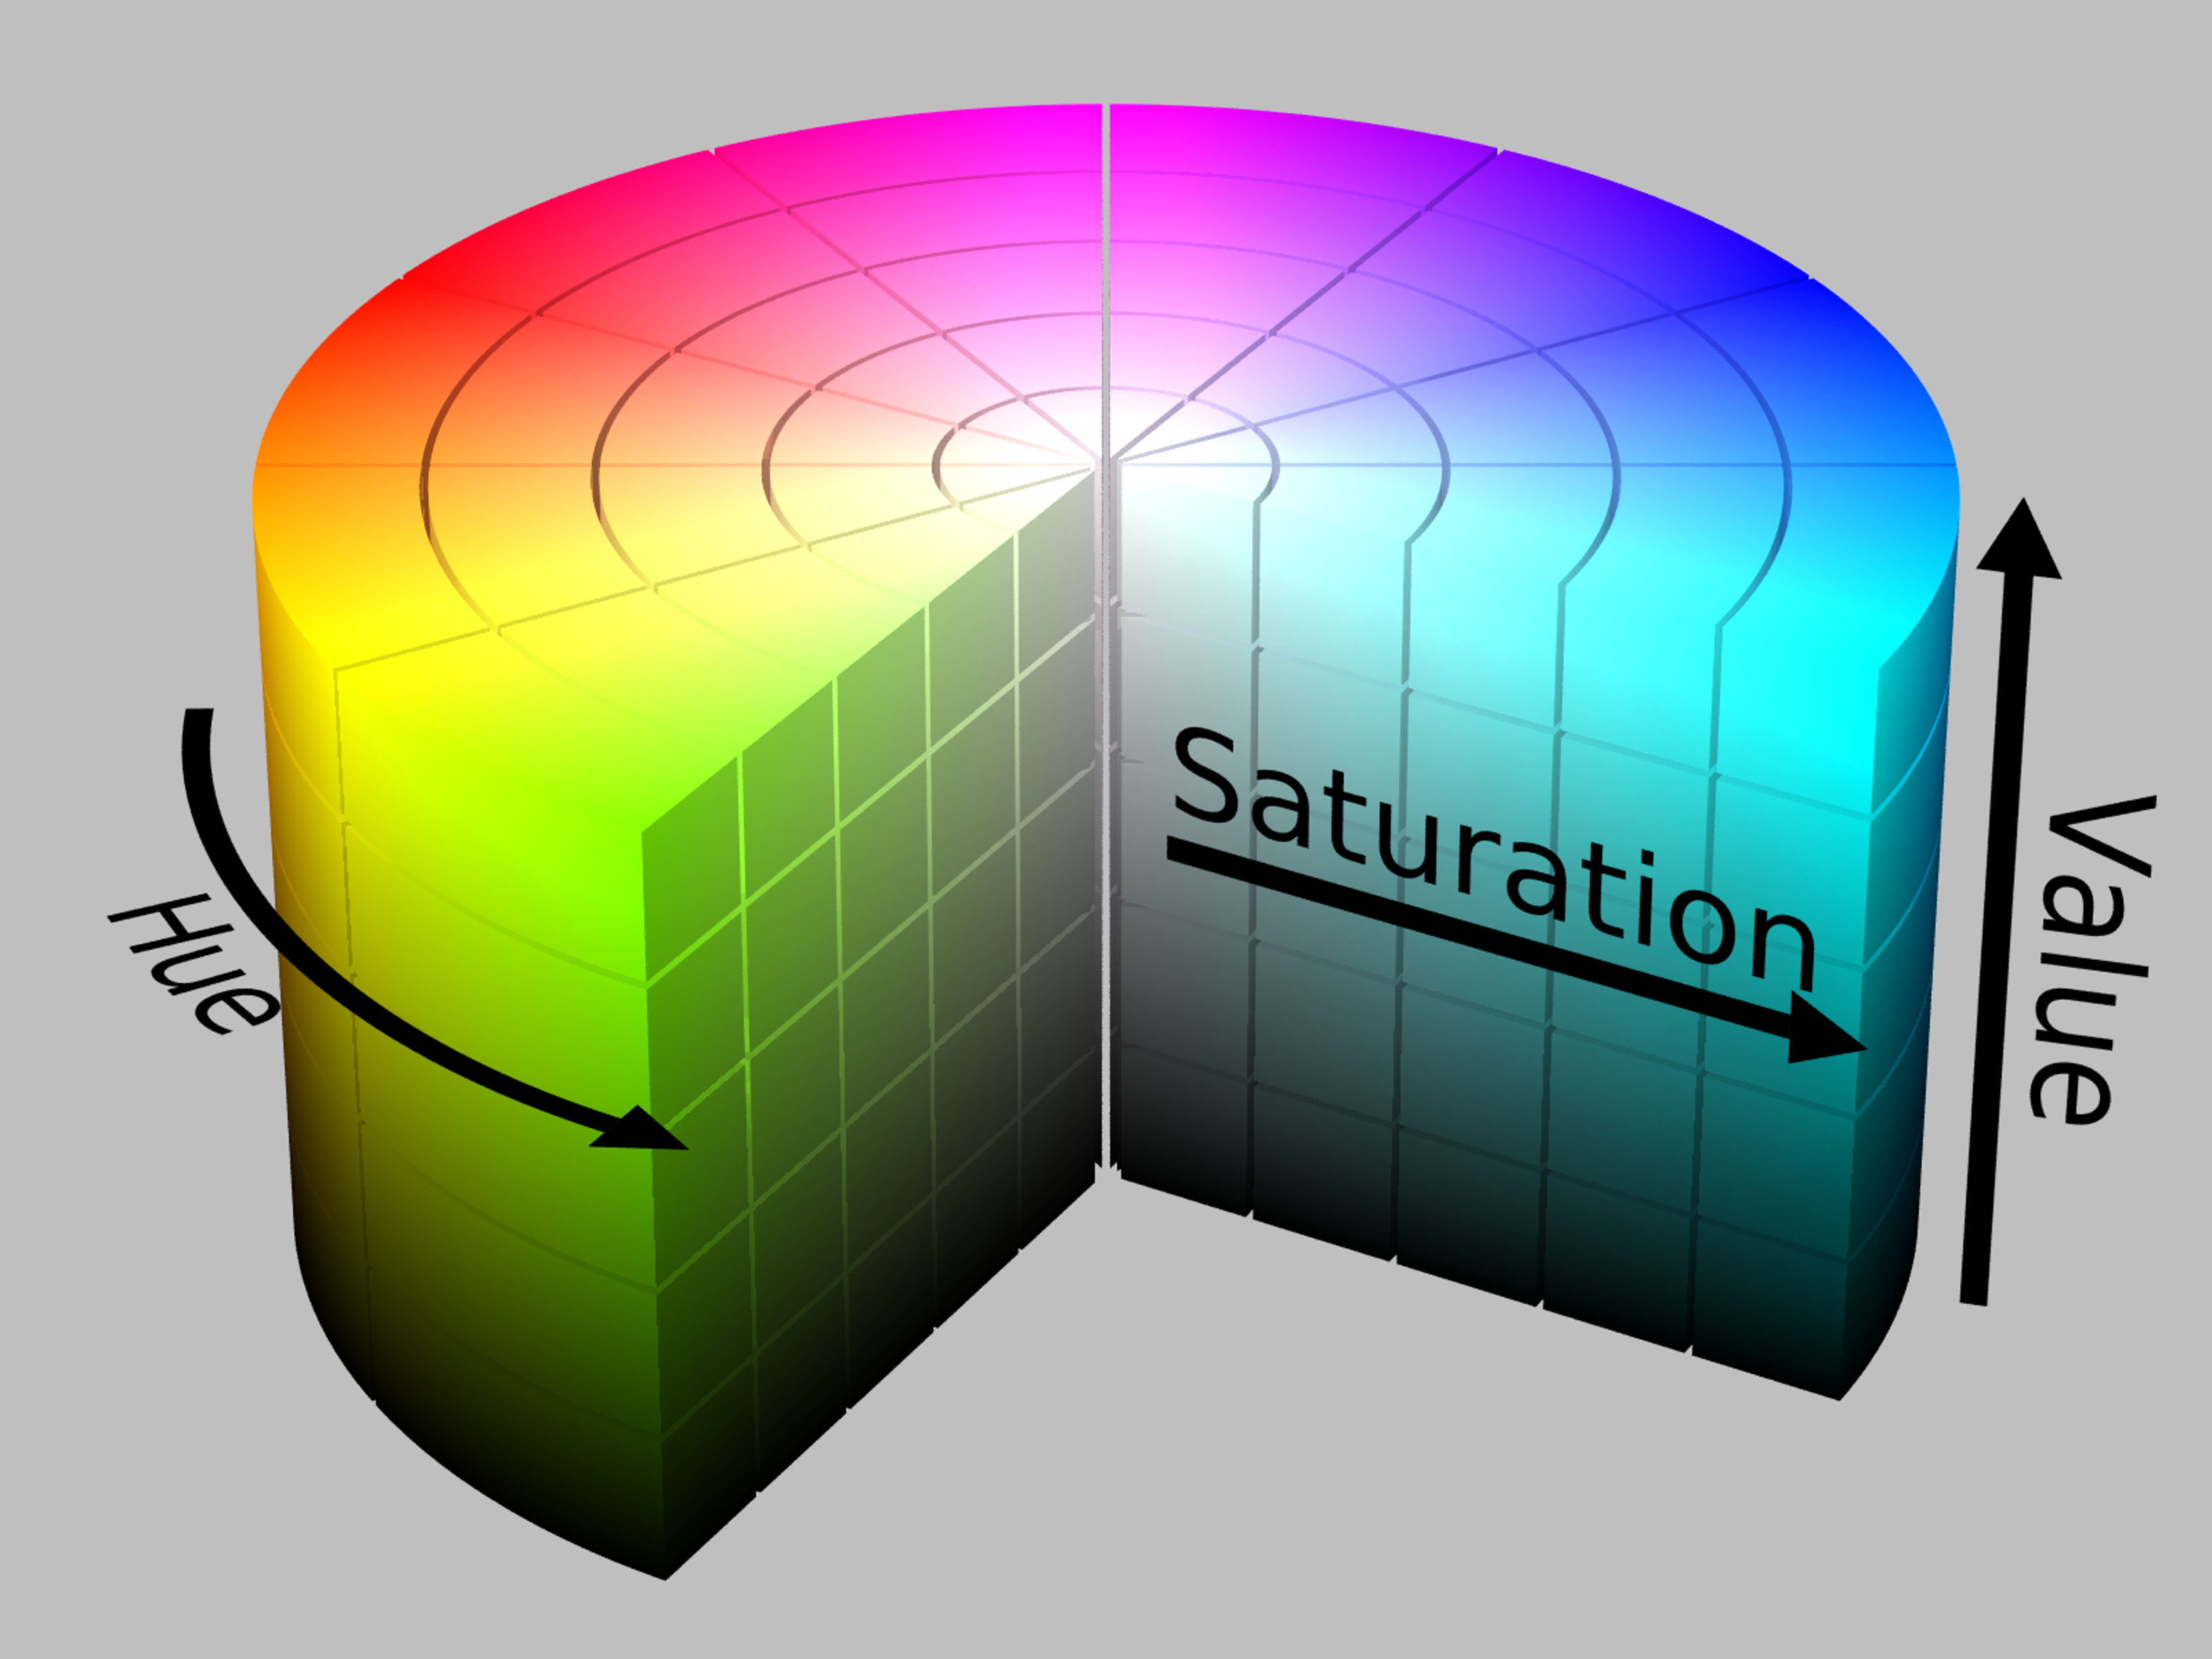
\includegraphics[width=0.48\textwidth]{hsv.pdf}
	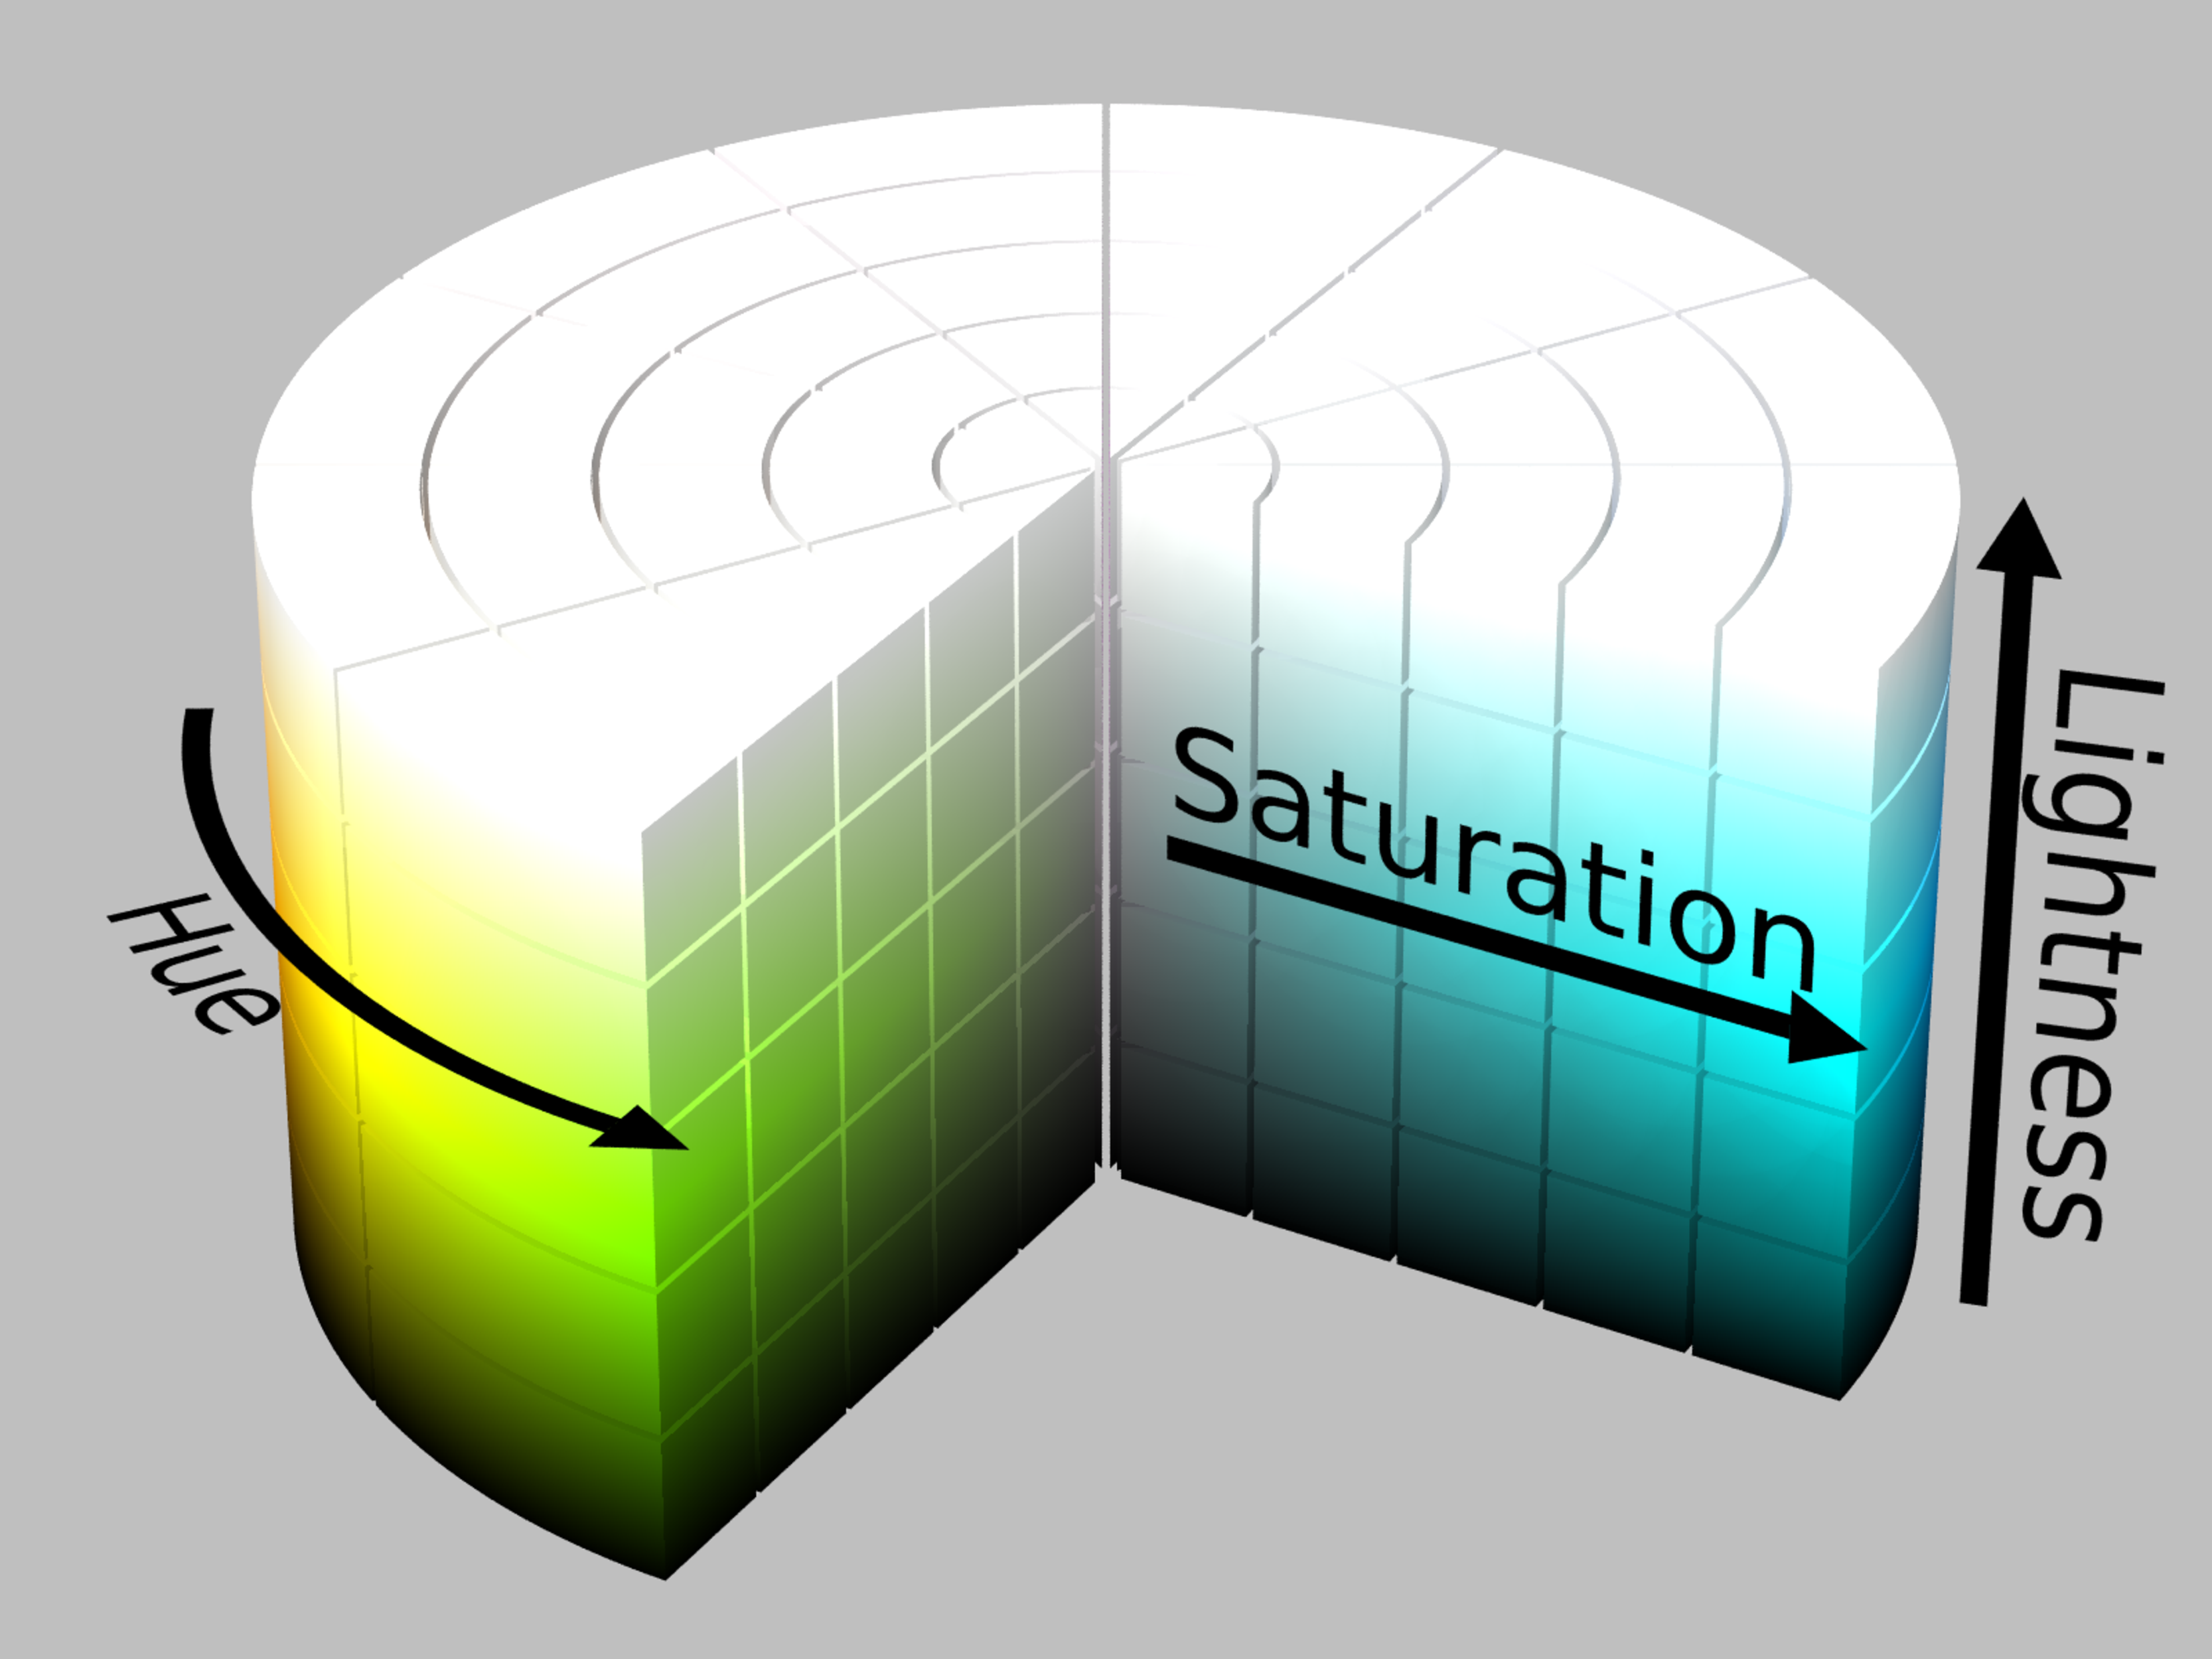
\includegraphics[width=0.48\textwidth]{HSL.pdf} \\
	(a) \hspace{10cm} (b)
	\caption{Exemplo do Modelo de Cor HSV(a) e HSL(b). Horvath\cite{ImagensHSLHSVRGB}}
	\label{ModeloHSV}
\end{figure} 
\subsubsection{HPG} 

O modelo de cores HPG foi proposto em 2007 pela Universidade Federal do Rio Grande do Norte estes partiram do princípio de que as cores podem ser definidas com uma mistura de cor pura e tom de cinza\cite{Martins:2007} e este é apropriado para aplicações onde seja necessário distinguir entre regiões de cor e regiões de cinza\cite{Mendes:2008}. O modelo define tonalidade (hue), pureza (purity) e cinzeamento (grayness). Neste modelo um pixel e definido como sendo composto por uma componente de cor pura e por uma componente de tom de cinza puro, ponderados por um fator de pureza\cite{Mendes:2008}.
O modelo de cores HPG se baseia nos valores obtidos de cada pixel no modelo RGB e então é feito um calculo de conversão.
\begin{figure}[!h]
	\centering
	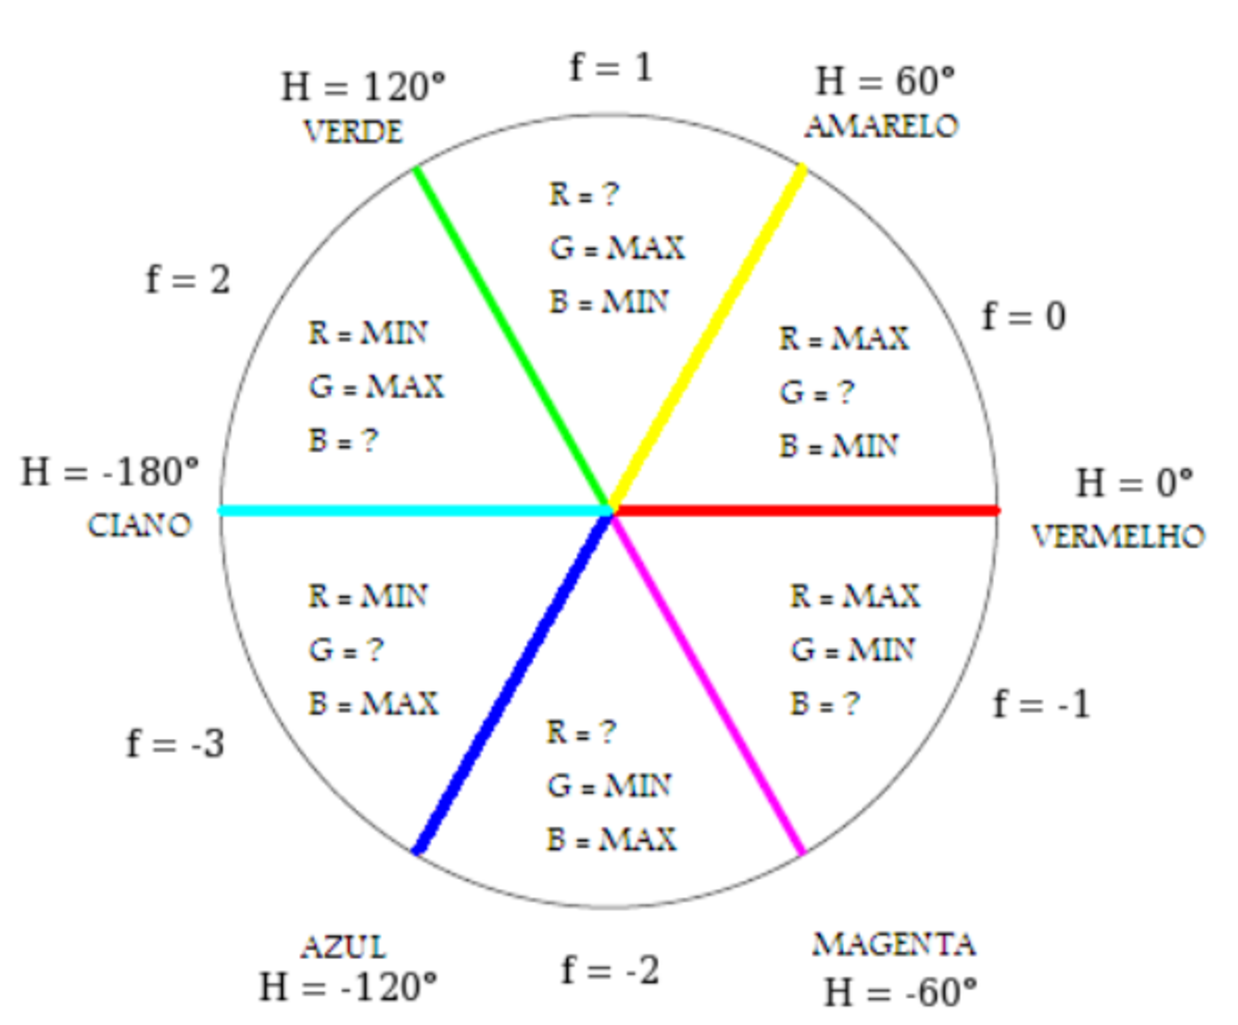
\includegraphics[width=0.48\textwidth]{hpg.pdf}
	\caption{Exemplo do Modelo de Cor HPG.  Mendes \cite{Mendes:2008}}
	\label{ModeloHPG}
\end{figure} 
\newpage
\section{Linguagem de Programação e Bibliotecas}


Para realização deste trabalho, irei utilizar a biblioteca de processamentos de imagens conhecida como OpenCV: Open Source Computer Vision Library. O trabalho será elaborado na linguagem C++, com uso do framework Qt para sua interface gráfica.
Os passos detalhados do projeto e seu desenvolvimento estará presente no Capítulo de Metodologia.
\begin{description}
	\item[OpenCV] Lançado em 1999 pela Intel\cite{Culjak:2012}, com objetivo de ser otimizada, portável e com um grande número de funções, o Open Source Computer Vision Library,OpenCV, se tornou se tornou uma ferramenta que possui mais de 2500 algoritmos e 40 mil pessoas em seu grupo de usuários\cite{Culjak:2012}. Já possui interface para as linguagens C++, C, Python e Java além de suporte para as principais plataformas com Windows, Linux, Mac OS, iOS e Android. A biblioteca lida tanto com imagens em tempo real, como vídeos e imagens estáticas.
	
	\item[Qt] Qt é um framework de desenvolvimento de aplicações multiplataforma. Entre suas funcionalidades está a possibilidade de criar interfaces gráficas diretamente em C ++ usando seu módulo Widgets.
	
	\item [C++] A linguagem de programação C++ foi projetado por Bjarne Stroustrup para fornecer eficiência e flexibilidade da linguagem C para programação de sistemas. A linguagem evoluiu a partir de uma versão anterior chamado C com Classes, o projeto C com Classes durou entre 1979 e 1983 e determinou os moldes para o C++. A linguagem foi oficialmente lancada em 1986.\cite{Stroustrup:1996} 
\end{description}


\section{Probabilidade e Estatística}

Para a automatização dos sistema de detecção de bordas e objetos foi utilizado a Distribuição T de Student para encontrar o valor de referencia \textit{t} para encontrar a Tabela T\cite{TabelaUFF} para assim calcular o valor do Intervalo de Confiança, usado para limitar o tamanho desejado dos objetos.
Todas as definições dessa seção foram retidas do livro Estatística de Spiegel\cite{Spiegel:1974}. 
\subsection{T de Student}
Com a necessidade de manipular dados de pequenas amostras William Sealey Gosset com o pseudônimo de Student derivou o teste t de Student baseado na distribuição de probabilidades t, publicando esses estudos em 1908 na revista Biometrika\cite{UFRN}.
A teoria T de Student é um teoria usada em pequenas amostras, ou seja, amostras com tamanho menor que 30.

De acordo com Spiegel \cite{Spiegel:1974}, a definição da distribuição de "Student" t é dada por:
\begin{displaymath} 
\textit{t}= \frac{\bar{X} - \mu }{\textit{s}} \sqrt{N - 1} = \frac{\bar{X} - \mu}{  \hat{s} / \sqrt{N} }
\end{displaymath}

Considerando-se amostras de tamanho N, extraídas de uma população normal de média  $\mu$, e, se para cada amostra cacular-se o valor de \textit{t}, por meio da média amostral e $\bar{X}$ e do desvio padrão s ou $\hat{s}$, pode-se obter a distribuição amostral de \textit{t}.
\begin{figure}[!h]
	\centering
	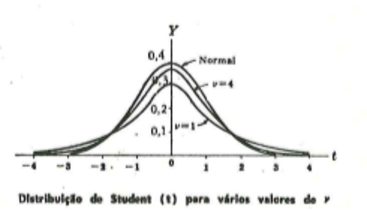
\includegraphics{distt.pdf}
	\caption{Distribuição de Student(t) para valores de v.  Spiegel \cite{Spiegel:1974}}
	\label{DistribuicaoTparV}
\end{figure}

\newpage
A distribuição(figura 2.5) é dada por:
\begin{displaymath}
Y=\frac{Y_{0}}{\left ( 1 + \frac{\mathit{t}^{2}}{N-1} \right ) ^{N/2}} = \frac{Y_{0}}{\left ( 1 + \frac{\mathit{t}^{2}}{\nu} \right ) ^{\left (\nu+1  \right )/2}}
\end{displaymath}
em que Y$_0$ é uma constante que depende de N, de modo que a Área subentendida pela curva é igual a 1, e que a constante  $\nu$ = (N - 1) é denominada \textit{número de graus de liberdade $\nu$}.
\subsection{Graus de Liberdade}
O numero de graus de liberdade é definido como o número N de observações independente da amostra, menos o numero \textit{k} de parâmetros populacionais que devem ser estimados por meio das observações amostrais. Simbolicamente, $\nu$ = N - \textit{k}.
O numero de graus de liberdade para a Distribuição T de Student é definida pelo número de observações independentes da amostra N, do qual podem ser calculados $\bar{X}$ e \textit{s}. Entretanto, como $\mu$  deve ser avaliado, k =1, então, $\nu$ = N-1.


\subsection{Intervalos de Confiança}

A estimativa de parâmetro dada por dois números é denominada \textit{estimativa por intervalo}, esta estimativa é considerada mais precisa e exata e assim é preferível à outras estimativas. Se a distribuição é aproximadamente normal pode se esperar que se encontre uma estatística amostral real, situada nos intervalos, assim pode-se esperar, ou estar confiante, de que o valor seja encontrado entre os intervalos, por esse motivo, esses intervalos são considerados intervalos de confiança. Para fazer o calculo dos Intervalos de Confiança é necessário escolher o \textit{Nível de Confiança}, dados em percentagem e que ficam, na maioria dos casos, entre 95\% e 99\%.

Os limites do Intervalo de Confiança para médias, pode ser representado por:
\begin{displaymath}
\bar{X}  \pm \mathit{t}_{\mathit{c}}\frac{\mathit{s}}{{\sqrt{N-1}}}
\end{displaymath}
onde os valores, dos limites iniciai e final, \textit{t$_c$} são denominados \textit{críticos} ou \textit{coeficiente de confiança} e dependem do nível de confiança desejado e do tamanho da amostra. Valores retirados da Tabela T, neste trabalho foi usada para referencia a Tabela T da Universidade Federal Fluminense\cite{TabelaUFF}. Para os propósitos finais foi escolhido um nível de confiança de 95%.
\section{Futebol de Robôs}
 Visto como um dominio bastente complexo, dinamico e imprevisivel\cite{Costa:2000}, o futebol de robos surgiu como uma tentativa de promover pesquisas nos campos de Inteligencia Artificial e robotica, pela avaliacao teorias, algoritmos e arquiteturas atraves problemas padrao\cite{Kitano:1997}.
 A Equipe Cedro se enquadra na categoria IEEE Very Small Size. Esta categoria é regulamentada pelo Instituto de Engenheiros Eletricistas e Eletrônicos (IEEE) e possui regras baseadas na MiroSot\cite{Rosa:2015}. O futebol de robos se assemelha ao futebol humano onde o objetivo do jogo é fazer gols para vencer a partida, porem tendo regras adaptadas para o "ambito" robotico. 
 Rosa\cite{Rosa:2015} em seu trabalho de graduação faz uma boa enumeração das regras básicas:
 \begin{itemize}
 \item A partida dura 10 minutos com dois tempos de 5 minutos;
  \item Há um intervalo de 10 minutos entre um tempo e outro;
   \item Cada time tem direito a dois tempos de 2 minutos que podem ser pedidos a qualquer
   momento;
    \item Caso a diferença de gols entre os dois times chegue a 10 a partida é encerrada;
     \item Uma falta ocorre quando há mais de um robô de um mesmo time dentro de sua própria
     área de gol ou quando um robô empurrar outro robô de outro time;
     \item Um pênalti ocorre quando a bola fica mais de 10 segundos dentro de alguma das áreas;
     \item Um chute-livre ocorre quando os robôs ficam travados por mais de 10 segundos, caso
     ocorra, o juiz posiciona a bola na marca de chute-livre mais próxima de onde ela ficou
     parada e posiciona os robôs de cada time equidistantes a bola;
     \item A cada inicio de partida ou gol feito a bola deve ser posicionada no centro do campo e os
     robôs devem ser posicionados de acordo com a posse de bola.
 \end{itemize}
\section{Trabalhos Relacionados}
Para o tema especifico deste trabalho, calibração de intervalo de cores para times de futebol de robos da categoria very small size, não foram encontrados trabalhos relacionados, porém foram encotrados Team Discription Papers e descrições de sistemas usados pelos times, onde consta sobre o processo de calibração e os metodos usados.

\subsection{Calibra}
O Centro Universitário da FEI, como visto em\cite{PenharbelTime}, utiliza em sua equipe Y04 utiliza um sistema, desenvolvido denominado CALIBRA\cite{Penharbel:2004}.Desenvolvido para sistemas Linux e com Graphical User Interface\cite{Penharbel:2004}, o sistema de calibração possui um modulo chamado de MainWindow, que é responsavel pela configuracao de brilho, cor e contraste da imagem adquirida pela camera e gera um arquivo que é analizado na hora da criacao das cores padrao\cite{PenharbelTime}, onde cores-padrão são definidas como intervalos no espaço de cores HSI\cite{PenharbelTime}.
\newpage
\begin{figure}[!h]
	\centering
	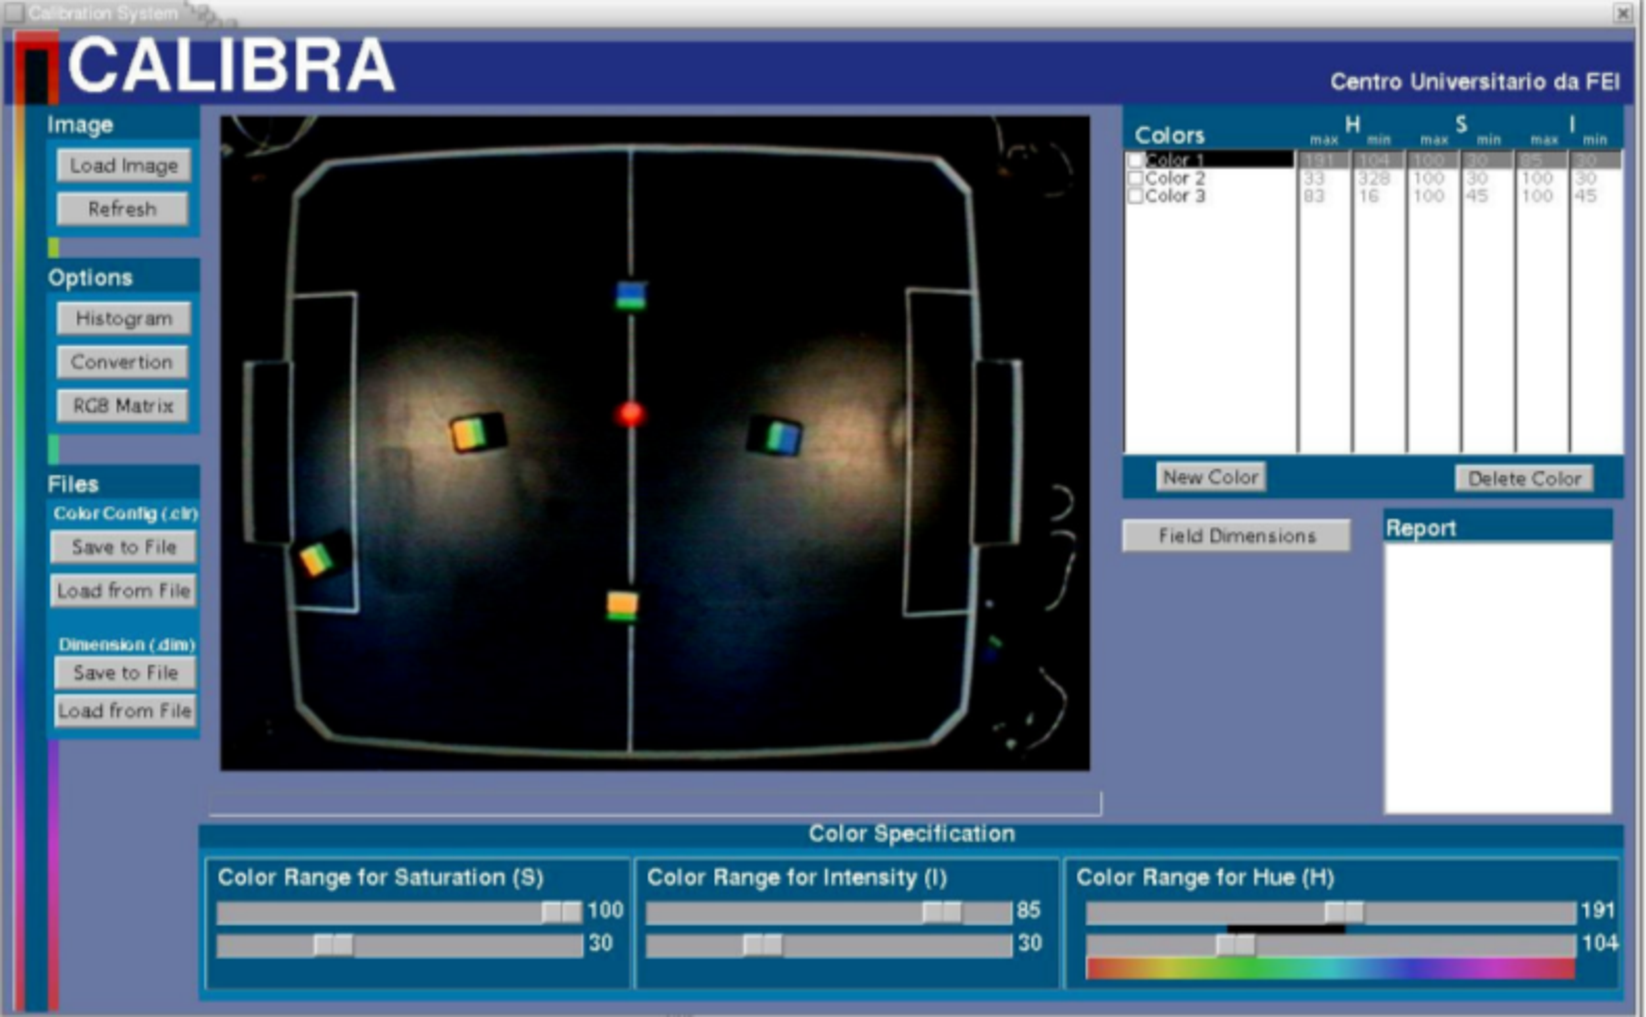
\includegraphics[width=0.6\textwidth]{calibra.pdf}
	\caption{Sistema Calibra desenvolvido pelo Centro Universitário da FEI \cite{Penharbel:2004}}
	\label{Calibra}
\end{figure}




\newpage
\subsection{VSS-Vision}
Desenvolvido inicialmente em Janeiro de 2016 pelo Laboratório de Sistemas Inteligentes de Robótica (SIRLab), utilizando para procesamento de imagens a biblioteca OpenCV e para telas interativas a biblioteca  ImGui.

\begin{figure}[!h]
	\centering
	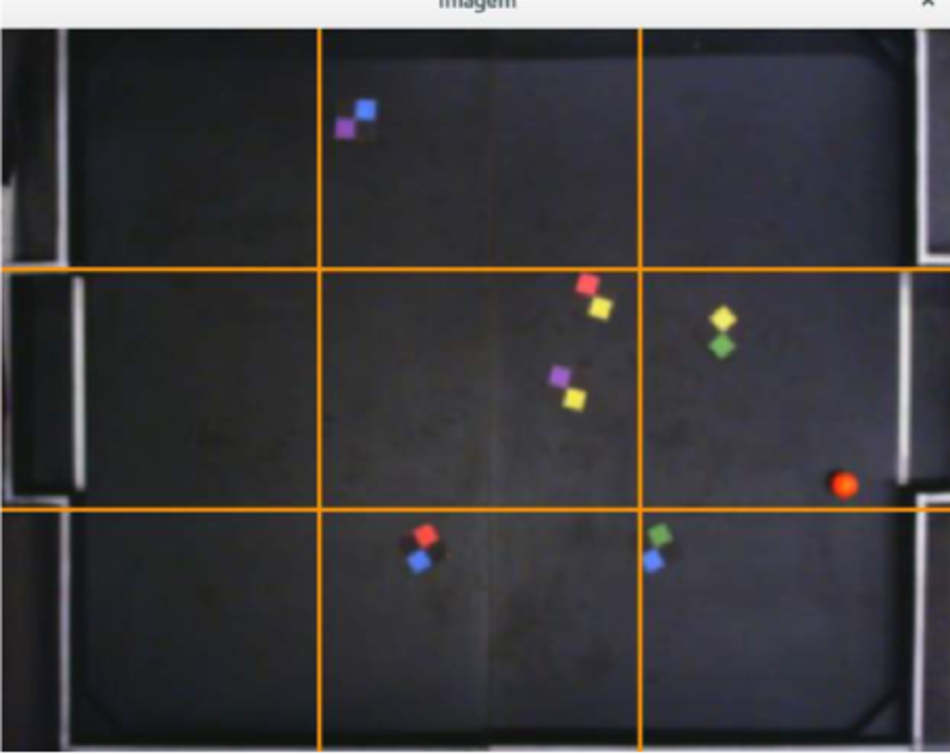
\includegraphics[width=0.4\textwidth]{vssvision.pdf} 	
	\caption{Sistema de calibracao desenvolvido peloSIRLab \cite{Rosa:2015}}
	\label{SIRLabCalibracao}
\end{figure}

A rotina de calibração do VSS-Vision calibra laranja, amarelo e azul obrigatoriamente e as outra cores referentes aos jogadores em campo\cite{Rosa:2015} de acordo com a escolha do time. A imagem é divida em nove cantos, como visto na imagem 2.7, e para calibrar a cor o usuario deve clicar em cima da cor que gostaria de ser calibrada salvando um intervalo de cor tratado como RGB máximo daquela cor e o mínimo, a medida
que vão havendo os cliques o sistema verifica para cada atributo se ele é maior que o atributo
máximo salvo ou menor que mínimo salvo, caso seja, o mesmo assume o lugar de menor ou
maior\cite{Rosa:2015} e esse processo deve ser feito em cada um dos nove cantos da imagem. Os valores HSV encontrados sao ajustados manualmente com a ajuda de sliders, como visto na imagem 2.8.
\begin{figure}[!h]
	\centering
	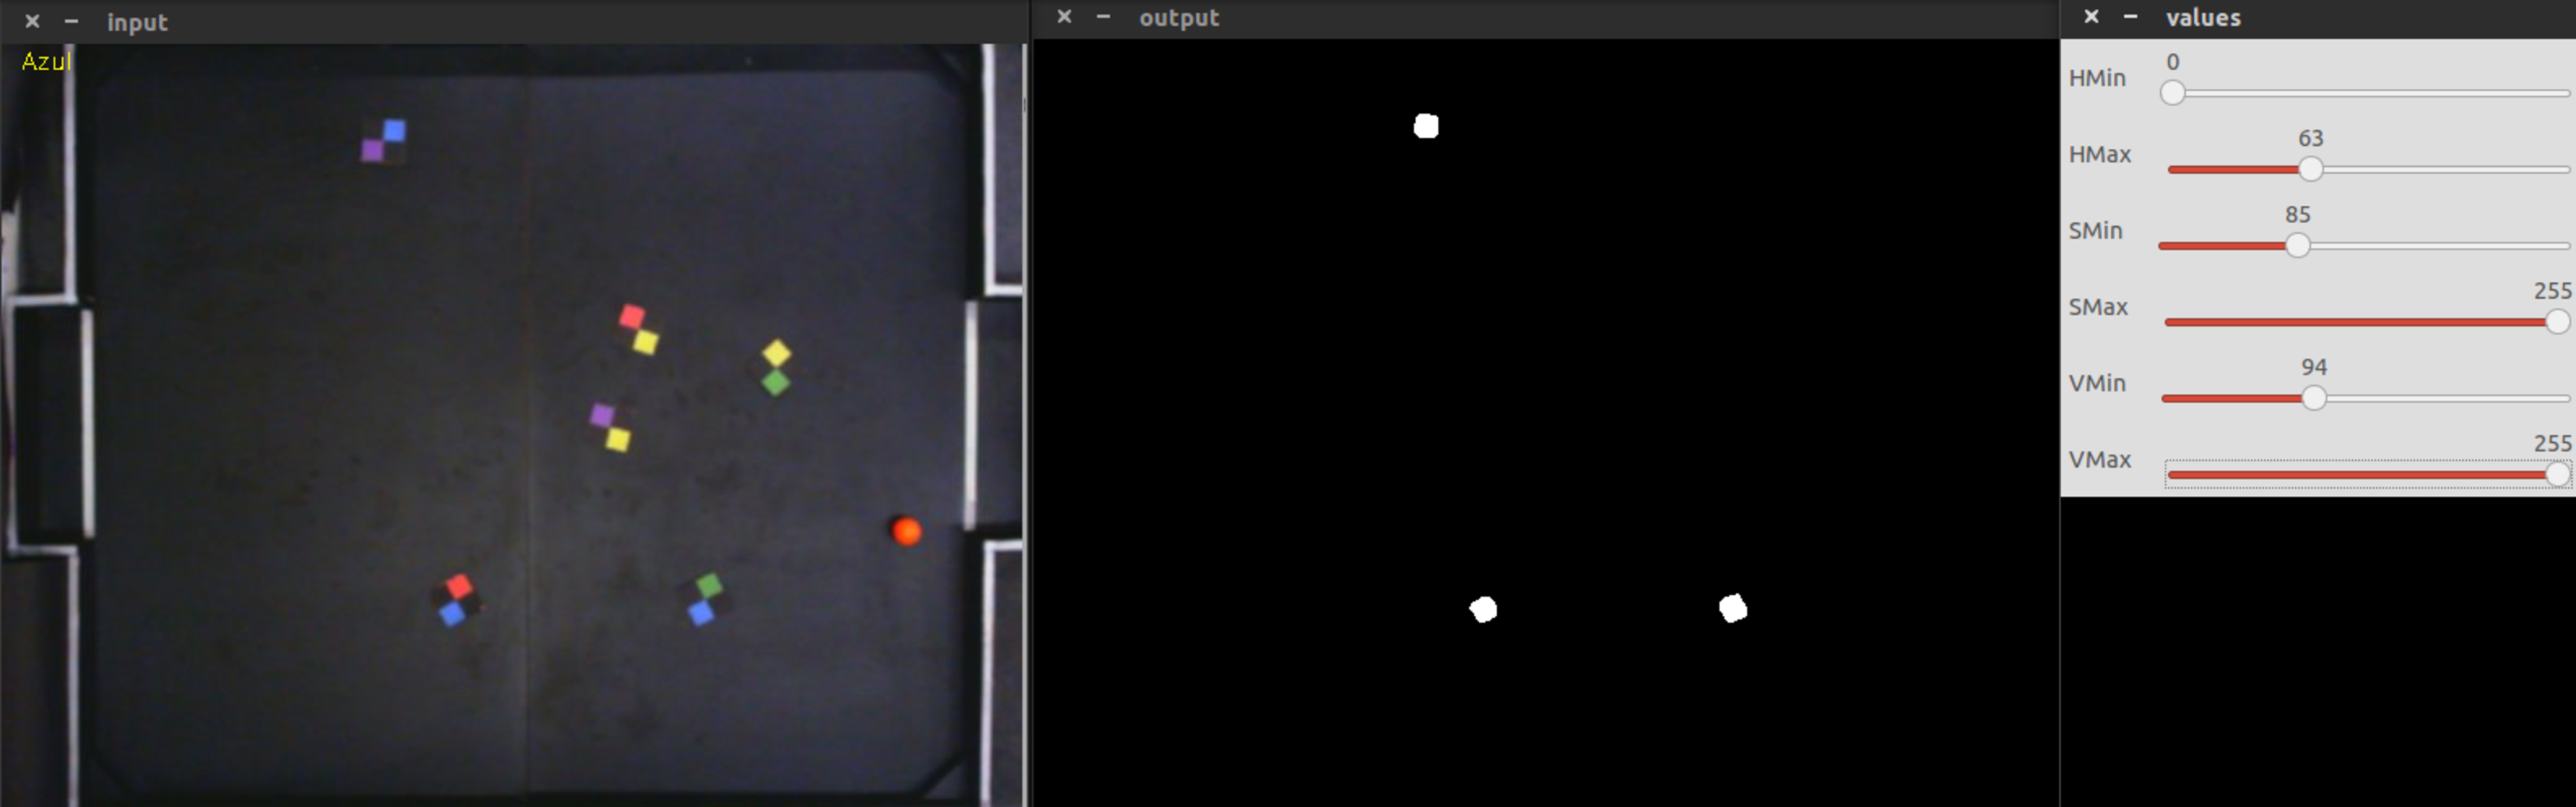
\includegraphics[width=0.8\textwidth]{calibration.pdf} 	
	\caption{Sistema de calibracao desenvolvido peloSIRLab \cite{VSSVision}}
	\label{SIRLabCalibracaoHSV}
\end{figure}
Por conta de ser feita manualmente, a calibraç~ao dura de 5 á 10 minutos
